\documentclass[12pt, letterpaper]{article}

\usepackage{enumitem}
\usepackage{amsmath}
\usepackage{graphicx}
\usepackage[margin=1in]{geometry}
\usepackage{cancel}
\usepackage{amssymb}
\usepackage{amsfonts}
\usepackage{amstext}
\usepackage{amsthm}
\usepackage{xcolor}
\usepackage{titlesec}
\usepackage{pgfplots}
\usepackage{mdframed}
\usepackage{nicefrac}
\usepackage{dsfont}
\usepackage{tikz}
\usetikzlibrary{trees}
\usepackage{mathdots}
\usepackage{accents}
\usepackage{mathtools}
\usepackage{bbm}

\usepackage{import}

\usepackage[T1]{fontenc}
\usepackage[utf8]{inputenc}
\usepackage{lmodern}
\usepackage[hidelinks]{hyperref}
\usepackage[T1]{fontenc}
\usepackage[utf8]{inputenc}

\usepackage[english]{babel}
\usepackage{csquotes}

\usepackage{xcolor}



\usepackage[notes,backend=biber]{biblatex-chicago}

% theorem environments
\newtheorem{theorem}{Theorem}
\newtheorem{lemma}{Lemma}
\newtheorem{corollary}{Corollary}

\theoremstyle{definition}
\newtheorem{definition}{Definition}
\newtheorem{example}{Example}

\theoremstyle{remark}
\newtheorem*{claim}{Claim}
\newtheorem*{remark}{Remark}
\newtheorem*{note}{Note}

\setlength{\textwidth}{6.0in}
\setlength{\oddsidemargin}{0in}
\setlength{\evensidemargin}{0in}
\setlength{\topmargin}{-0.5in}
\setlength{\headheight}{0.25in}
\setlength{\headsep}{0.25in}
\setlength{\textheight}{8.5in}
\setlength{\footskip}{20pt}

\setlength{\topskip}{0in}

\setcounter{secnumdepth}{0}

\setlength{\parindent}{0in}	
\setlength{\parskip}{0.1in}

\newcommand{\vect}[1]{\vec{\mathbf{#1}}}
% \newcommand{\sectionbreak}{\clearpage}
\newcommand{\R}{\mathbb{R}}
\newcommand{\Z}{\mathbb{Z}}
\newcommand{\N}{\mathbb{N}}
\renewcommand{\P}{\mathbb{P}}
\newcommand{\F}{\mathbb{F}}
\newcommand{\modop}{\;\text{mod}\;}
\renewcommand{\mod}[1]{\;(\text{mod}\;#1)}
\newcommand{\Aut}{\text{Aut}}
\newcommand{\id}{\text{id}}
\newcommand{\spn}{\;\text{span}}

\DeclareMathOperator*{\argmax}{argmax}

\newcommand{\ftntmk}{\textcolor{blue}{\footnotemark}}
\newcommand{\black}[1]{\textcolor{black}{#1}}
\newcommand{\ubcolor}[2]{\color{#1}{\underbrace{\color{black}{#2}}}}
\newcommand*\circled[1]{\tikz[baseline=(char.base)]{
            \node[shape=circle,draw,inner sep=2pt] (char) {#1};}}

\newcommand{\vol}[1]{\text{vol}}

\newcommand{\verteq}{\rotatebox{90}{$\,=$}}
\newcommand{\equalto}[2]{\underset{\scriptstyle\overset{\mkern4mu\verteq}{#2}}{#1}}

\newcommand{\rk}{\text{rk}\,}
\newcommand{\Col}{\text{Col}\,}
\newcommand{\C}{\mathbb{C}}
\newcommand{\Q}{\mathbb{Q}}
\newcommand{\actson}{\curvearrowright}

\newcommand{\E}{\mathbb{E}}

\renewcommand{\mapsto}{\longmapsto}

% James - Parentheses, brackets, etc.
\newcommand{\ignore}[1]{}  % from Charles
\newcommand{\parens}[1]{\ensuremath{\left( #1 \right)}}
\newcommand{\bracks}[1]{\ensuremath{\left[ #1 \right]}}
\newcommand{\braces}[1]{\ensuremath{\left\{ #1 \right\}}}
\newcommand{\angbrs}[1]{\ensuremath{\langle #1 \rangle}}
\newcommand{\set}[1]{\braces{#1}}
\newcommand{\powset}[1]{\mathcal{P}\parens{#1}}
\newcommand{\vspan}[1]{\angbrs{#1}}  % 4330: Span of a set of vectors

\newcommand{\floor}[1]{\left\lfloor #1 \right\rfloor}
\newcommand{\ceil}[1]{\left\lceil #1 \right\rceil}
\newcommand{\verts}[1]{\left\lvert #1 \right\rvert} % | #1 |
\newcommand{\Verts}[1]{\left\lVert #1 \right\rVert} % || #1 ||
\newcommand{\abs}[1]{\verts{#1}}
\newcommand{\size}[1]{\verts{#1}}
\newcommand{\norm}[1]{\Verts{#1}}

\newcommand{\eps}{\varepsilon}
\newcommand{\vphi}{\varphi}
\renewcommand{\Re}{\mathrm{Re}}
\renewcommand{\Im}{\mathrm{Im}}

\newcommand{\bmat}[1]{\begin{bmatrix} #1 \end{bmatrix}}
\newcommand{\pmat}[1]{\begin{pmatrix} #1 \end{pmatrix}}

\bibliography{bibliography}

\title{ML Kit: A Machine Learning Library for Rust}

\author{Owen Wetherbee (ocw6), Ethan Ma (em834), Sylvan Martin (slm338)}
\date{}


% Body

\pgfplotsset{compat=1.16}
\begin{document}

\maketitle

\begin{center}
    \textbf{Keywords:} Machine learning, Gradient Descent, PCA, Rust
\end{center}

\subsubsection*{Application Setting}

Rust is a relatively new programming language with a dearth of machine learning infrastructure. We aimed to 
create a library for Rust programmers to make machine learning convenient, much like NumPy or TensorFlow in Python.

\section{Project Description}

Initially, we wanted to create a comprehensive machine learning library for Rust, which would use Rust's safety
and speed to implement many algorithms used in data science. We had the original (lofty) goal of being able to 
run a diffusion model by the end of the semester, or be able to do anything that NumPy/SciKitLearn could do. As 
we began implementation we recognized that we lacked the time and resources to implement the sheer amount of algorithms 
we set out to. So, we shifted our focus to what we believe are some of the core algorithms in the field of 
Machine Learning.

In the end, we created the pure-Rust library \texttt{ml\_kit}, which implements, from scratch, the following:
\begin{itemize}
    \item Neural Network based learning, consisting of
    \begin{itemize}
        \item the basic neural network model with user-defined network shape and activation functions 
        for each layer
        \item functionality for handling large datasets for training and testing
        \item a stochastic gradient descent trainer, with whatever batch size and epochs a user may want
        \item various ``gradient update schedules,'' such as fixed learning rates, time-decay learning rates, AdaGrad, etc.
        \item Convolutional Neural Networks (Owen/Ethan talk more on this?)
    \end{itemize}
    \item Principle Component Analysis, consisting of
    \begin{itemize}
        \item an implementation of Singular Value Decomposition (SVD),
        \item using SVD to obtain a $k$-dimensional plane of best fit for a set of points in $\R^n$,
        \item compressing images (or any data) using SVD by truncating low-variance dimensions
    \end{itemize}
\end{itemize}

\subsection{Neural Networks}

\subsection{Principle Component Analysis and SVD}

Singular Value Decomposition (SVD) is a factorization of a matrix $A \in \R^{m \times n}$ into
\[
    A = U \Sigma V^\top
\]
where $U \in \R^{m \times m}$ and $V \in \R^{n \times n}$ are orthogonal matrices with 
columns $\vect u_1, \ldots \vect u_m$ and $\vect v_1, \ldots, \vect v_n$ respectively, and $\Sigma$
is a diagonal matrix of the form (assuming $n \leq m$)
\[
    \Sigma = \left[
        \begin{array}{cccc}
            \sigma_1 & & & \\
            & \sigma_2 & & \\
            & & \ddots & \\
            & & & \sigma_n \\
            & & & \\
            & & & 
        \end{array}
    \right] \in \R^{m \times n}
\]
where $\sigma_1 \geq \sigma_2 \geq \cdots \geq \sigma_n \geq 0$ are the \emph{singular values} of $A$.
This allows us to write $A$ as the linear combination
\[
    A = \sum_{i = 1}^n \sigma_i \vect{u}_i \vect{v}_i^\top
\]
Note that because the singular values are sorted in decreasing order, we can effectively ``save data'' in 
representing $A$ by truncating all but the first $r \leq n$ singular vectors, as the last items in the sum do not 
contribute as much to the 
overall product. The immediate application is identifying the most significant axes of correlation in data, allowing 
dimensionality reduction of datasets by re-writing each item in the basis $\vect{v}_1, \ldots, \vect{v}_r$.
Commonly, the ``data'' of concern is written into the rows of $A$.

\subsubsection{What we implemented}

Our library implements the Golub-Kahan SVD algorithm (described in ``Matrix Computations,'' by Golub and van Loan.
\textcolor{blue}{\autocite{golub13}}) which begins by bi-diagonalizing $A$, then performing SVD on the bidiagonalization,
as the numerical stability and performance are better. Once we were able to compute the SVD of any matrix, we could use 
SVD as a subroutine in other useful techniques.

The (subjectively) coolest application of SVD we implemented is image compression. By taking an $m \times n$ image and 
writing it as a 4-tuple of matrices $(R, G, B, A)$ representing the red, green, blue, and alpha channels of the pixels,
we can perform SVD on each color channel, store only the SVD representation after truncating insignificant singular
vectors, and then de-compress the image later by computing $U \Sigma V^\top$ for each color channel. In practice,
one can discard roughly half the singular values and still obtain a recognizeable image. Examples of this and discussion 
of runtime and compression rates will be left to the evaluation section.

A common goal in statistics is finding the ``line of best fit'' of a set of points, or in higher dimensions,
a $k$-dimensional plane of best fit. For a cluster of data centered at the origin, the first singular vector, $\vect v_1$,
is the line of best fit. This is because SVD is equivalently defined as an optimization proceedure where 
\[
    \vect v_1 = \argmax_{\|x\| = 1} \|Ax\|
\]
Since $\vect v_1$ is maximizing the sum of squares of the inner products with all the data points, it is minimizing 
the sum of squared distances from each data point to the line spanned by $\vect v_1$. More generally, taking the first 
$\vect v_1, \ldots, \vect v_k$ vectors, we obtain a basis for a $k$-dimensional ``plane of best fit.'' 

We implement a proceedure which takes a data matrix $D \in \R^{n \times m}$ whose columns are each $\R^n$ data points, 
and returns $\vect \mu \in \R^n$ and $V \in \R^{n \times k}$ such that the plane defined by 
\[
    \left\{\vect \mu + \sum_{i = 1}^{k} \alpha_i \vect v_i \mid \alpha_i \in \R\right\}
\]
is the plane of best fit for the data. Examples of this will be left to the evaluations section.

\subsection{Relationship to Other Work}

Linear algebra is the foundatin to machine learning, so we needed to use a good linear algebra library. Sylvan had 
previously spent winter break working on \texttt{matrix\_kit}, which is a pure-Rust linear algebra package that 
implemented incredibly basic matrix-vector operations. We continued developing this library in parallel with 
\texttt{ml\_kit} over the semester as we recognized more features that were needed from the linear algebra library. 
So, the sum of our work for the course can be thought of as the entirety of \texttt{ml\_kit}, as well as significant
improvement to the functionality of \texttt{matrix\_kit}.

The \texttt{matrix\_kit} library can be found on GitHub at \url{https://github.com/SylvanM/matrix_kit}.

\section{Evaluation}

\subsection{Gradient Descent}

\subsection{Principle Component Analysis}

In this section, we discuss the performance of our SVD-based algorithms in terms 
of their speed and correctness.

\subsubsection{Singular Value Decomposition}

\begin{center}
    \textbf{Correctness}
\end{center}

In numerical methods such as SVD, the accumulation of floating point error prevents us from measuring exact correctness.
Instead, we define some small $\varepsilon$, and consider two matrices $A \approx_\varepsilon B$ to be ``basically equal'' if 
for all $i, j$, $|a_{ij} - b_{ij}| < \varepsilon$. When testing on large matrices, we chose $\varepsilon = 1 \times 10^{-5}$
to be our goal, though in practice on smaller matrices ($m, n \leq 50$) we attain correctness up to $\varepsilon = 1 \times 10^{-9}$.

To test correctness of our SVD implementation, we start with a randomly generated matrix $A \in \R^{m \times n}$
where each entry is sampled from the normal distribution $\mathcal N(0, 1)$, and compute its SVD into $U$, $V$, 
and $\Sigma$. We then check that $U$ and $V$ are orthogonal by testing $U^\top U \approx_\varepsilon I_m$ 
and $V^\top V \approx_\varepsilon I_n$. We then check that $A \approx_\varepsilon U \Sigma V^\top$. 

Sometimes, our SVD implemention does not converge on a particular matrix, and so we abort the execution. The main loop 
of the Golub-Kahan algorithm should in theory take $\mathcal O(n)$ steps, so we introduced a check that if the main loop
runs more than $30n$ times, we declare the instance a failure, and return empty $0 \times 0$ matrices.

With $m$ and $n$ sampled randomly in the range $2$ through $20$, we ran the above testing proceedure 10,000 times and 
found no correctness failures, though we observe a divergence rate of about $2.49\%$. That is, on small matrices, our 
algorithm failed to converge on 249 out of the 10,000 random matrices.

The issue of convergence seems to become better with larger matrices. When we sample $m$ and $n$ randomly from the range 
$2$ through $200$, we found that out of 300 trials, only 1 instance failed to converge, a rate of $.33\%$.

For matrices with $200 \leq m, n \leq 300$, we found no matrices with failed to converge out of 30 trials.

\begin{center}
    \textbf{Runtime Performance}
\end{center}

Our SVD implementation is absurdly slow. It became impractical to test at a large scale for matrices with more than 
$500 \times 500 = 250,000$ entries. This is unfortunate, as most real-world applications would require much larger 
matrices. When we first tried image compression, we used a 4K image taken by an iPhone, and running SVD on 
each color channel took so long that even when let to run for 12 hours overnight, it didn't terminate. It is hard to 
know if this is because it genuinely just took so long, or if it fell into the small fraction of cases that caused 
divergence. Because of the decaying rate of divergence for larger dimensions, we believe it is the former. We also 
tried running SVD on matrices of comparable size (with $m$ and $n$ in the low thousands) and were unable to get 
it to terminate after several hours.

This is almost certainly due to the fact that at this stage of development we did \emph{not} fully optimize our 
Golub-Kahan implementation. The first step, which relies on bi-diagonalizing the matrix, uses a sequence of Householder 
reflections, which if implemented efficiently can take linear time as they only affect two rows of a matrix. Further 
optimization would include only applying the reflection to a sub-matrix of $A$, and not the entire matrix. Instead, 
we applied the householder reflection matrix to the entire matrix $A$, taking $\mathcal{O}(n^3)$ time for each step.
This easily balloons the runtime, since this is done inside an inner loop. At first, we tried implementing 
the fully optimized Golub-Kahan algorithm, but were unable to get it to work correctly. So, we focused on just 
trying to get a \emph{correct} implementation instead of premature optimization. The natural next steps after this 
project would be to get this running faster!

\subsubsection{Image Compression}

As discussed above, we were unable to run our image compression on large images, so we started with low-resolution 
images. We ran our image compression algorithm on two images, one of some sheep,\ftntmk{}\footnotetext{The 
sheep are in the teaching barn by the Vet School. I highly recommend that you go visit and pet them! It's 
free and you can just walk right up to them!}, and one 
of a cat. 

When a matrix $A$ is decomposed into $U, \Sigma, V$, and all but the first $k$ singular values are ditched, we are 
left with three matrices of sizes $m \times k$, $k$ and $n \times k$ (we need only store the diagonal of $\Sigma$).
So, the number of floating point values we must store as a fraction of the amount we would need to fully represent 
$A$ is what we call the ``compression ratio,'' computed as 
\[
    r = \frac{r + rm + rn}{mn}
\]
For small matrices and large values of $r$, this doesn't save much. However, this scales incredibly well for large matrices, 
as we can pick modestly small values of $r$ and end up with impressive compression ratios while still being able to recognize 
the original image. A small caveat here is that typically a single pixel's channel for one color only uses one byte to 
represent it, whereas we are using 64-bit floating points, so one could argue that we need to include a factor of 8 
in our compression ratio. However, our compression would work just as well if each color channel was represented 
as a floating point value between 0 and 1 (since this is what we convert the image to anyway when we begin 
compression), so we think it is fair to compare the sizes when thinking of the original channel as being a 
decimal between 0 and 1 as opposed to an integer between 0 and 255.

\begin{center}
    \textbf{Sheep}
\end{center}

We used a $240 \times 320$ pixel image of some sheep laying in a barn, and truncated the singular values
up to the first $k \in \{100, 50, 10\}$. Running SVD to decompose the image took \textbf{1m 15s}.

\begin{figure}[h]
	\centering
	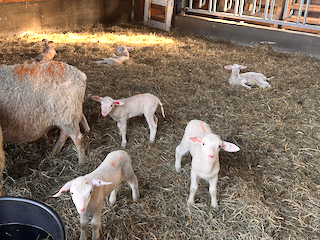
\includegraphics{images/sheep.png}
	\caption{The original image}
	\label{fig:sheep}
\end{figure}

\begin{center}
    \textbf{Panini (the cat)}
\end{center}

On a $640 \times 480$ image of Panini, SVD took \textbf{20m 50s} to finish, 

\subsubsection{Planes of Best Fit}




\printbibliography

\end{document}